\documentclass[aspectratio=169]{beamer}

% --- PACKAGES ---
\usepackage[english]{babel}
\usepackage{graphicx}
\usepackage{booktabs}
\usepackage{tcolorbox}
\usepackage{fontspec}
\usepackage{caption}
\captionsetup[figure]{labelformat=empty}
\usepackage{xcolor}
\usepackage{tikz} % Needed for \tikz \path commands
\usepackage{csquotes}
\usepackage{listings}
\usepackage{booktabs}
\usepackage{amsmath}
\usepackage{amssymb}
\usepackage{array}
\usepackage{graphicx}
\usepackage{colortbl}
\usepackage{tikz}

\usepackage[backend=biber, style=apa, doi=true]{biblatex}



% COLOR DEFINITIONS (KIT & HMC)
\definecolor{KITBlue}{RGB}{0, 98, 148}
\definecolor{HMCBlue}{RGB}{0, 40, 100}
\definecolor{HMCAccent}{RGB}{20, 200, 255}
\definecolor{HMCMint}{RGB}{5, 229, 186}
\definecolor{HMCClaim}{RGB}{0, 128, 64}
\definecolor{LightGray}{RGB}{242, 242, 242}
\definecolor{VeryLightGray}{RGB}{252, 252, 252}



% THEME APPLICATION (Minimalist)
\usefonttheme{professionalfonts}
\useinnertheme{default}
\useoutertheme{miniframes} % Minimalist header
% \setbeamertemplate{navigation symbols}{} % No navigation symbols

% Custom Footline Definition to insert the logo
\setbeamertemplate{footline}{
  \leavevmode
  \hbox{
    % Right box: Logo and Frame Number
    \begin{beamercolorbox}[wd=\paperwidth,ht=2.25ex,dp=1ex,right]{date in head/foot}
        \raisebox{-0.96 ex}{
\includegraphics[width=14ex]{figs/kit_logo_S5_02_rdax_98s.jpg}}|
        \raisebox{-0.14 ex}{
\includegraphics[width=10ex]{figs/hmc_logo.png}}| 
        \usebeamerfont{date in head/foot}\insertframenumber\hspace*{8ex}
    \end{beamercolorbox}}
    \vskip1ex
}

% 3. BEAMER COLOR SCHEMES
\setbeamercolor{palette primary}{fg=white, bg=HMCBlue}
\setbeamercolor{section in head/foot}{fg=white, bg=HMCBlue}
\setbeamercolor{palette secondary}{fg=white, bg=HMCAccent}
\setbeamercolor{structure}{fg=HMCAccent}
\setbeamercolor{local structure}{fg=HMCAccent}
\setbeamercolor{title}{bg=HMCBlue, fg=LightGray}
\setbeamercolor{frametitle}{fg=HMCBlue, bg=white}
\setbeamercolor{block title}{fg=HMCClaim, bg=LightGray}
\setbeamercolor{block body}{fg=HMCBlue, bg=VeryLightGray}
\setbeamercolor{author in head/foot}{bg=white, fg=HMCBlue}
\setbeamercolor{title in head/foot}{bg=white, fg=HMCBlue}
\setbeamercolor{date in head/foot}{bg=white, fg=HMCBlue}

% 4. FONT CONFIGURATION
% (Requires Noto Sans to be installed on your system)
%% \setmainfont{Noto Sans} 
%% \setsansfont{Noto Sans}
\lstdefinelanguage{XML}{
    basicstyle=\ttfamily\tiny,
    showstringspaces=false,
    breaklines=true,
    frame=lines,
    literate={>}{{{\color{HMCAccent}>}}}1
             {<}{{{\color{HMCAccent}<}}}1
}
\lstdefinelanguage{yaml}{
    basicstyle=\ttfamily\tiny,
    showstringspaces=false,
    breaklines=true,
    frame=lines,
    literate=
   % {  }{
   %   \makebox[0.5em][l]{\colorbox{HMCMint}{\phantom{p}}}
   %   \makebox[0.5em][l]{\colorbox{HMCMint}{\phantom{p}}}
   % }{2}
             {,}{{{\color{HMCAccent},}}}1
             {:}{{{\color{HMCAccent}:}}}1
             {[}{{{\color{HMCAccent}{[}}}}1
             {]}{{{\color{HMCAccent}{]}}}}1
             {\{}{{{\color{HMCAccent}{\{}}}}1
             {\}}{{{\color{HMCAccent}{\}}}}}1
}
\lstdefinelanguage{json}{
    basicstyle=\ttfamily\tiny,
    showstringspaces=false,
    breaklines=true,
    frame=lines,
    literate={"}{{{\texttt{\char34}}}}1
             {,}{{{\color{HMCAccent},}}}1
             {:}{{{\color{HMCAccent}:}}}1
             {[}{{{\color{HMCAccent}{[}}}}1
             {]}{{{\color{HMCAccent}{]}}}}1
             {\{}{{{\color{HMCAccent}{\{}}}}1
             {\}}{{{\color{HMCAccent}{\}}}}}1
}
\lstdefinelanguage{CSV}{
    basicstyle=\ttfamily\tiny,
    showstringspaces=false,
    breaklines=true,
    frame=lines,
    literate={,}{{{\color{HMCAccent},}}}1
    {;}{{{\color{HMCAccent};}}}1, 
}

% 5. Define the switch \ifenablepauses
\newif\ifenablepauses
% Set the default state
\enablepausestrue           % (for animated presentation)
\enablepausesfalse          % (for static presentation)



\title{How to Automatise Data Description and Publication}
\subtitle{Transformation of Data Management Plans to a FAIR Annotation of Datasets}
\author{A. Koubaa}
\date{\today}

\begin{document}

\begin{frame}
\titlepage
\end{frame}

\begin{frame}{EDO Overview}
    \begin{center}
    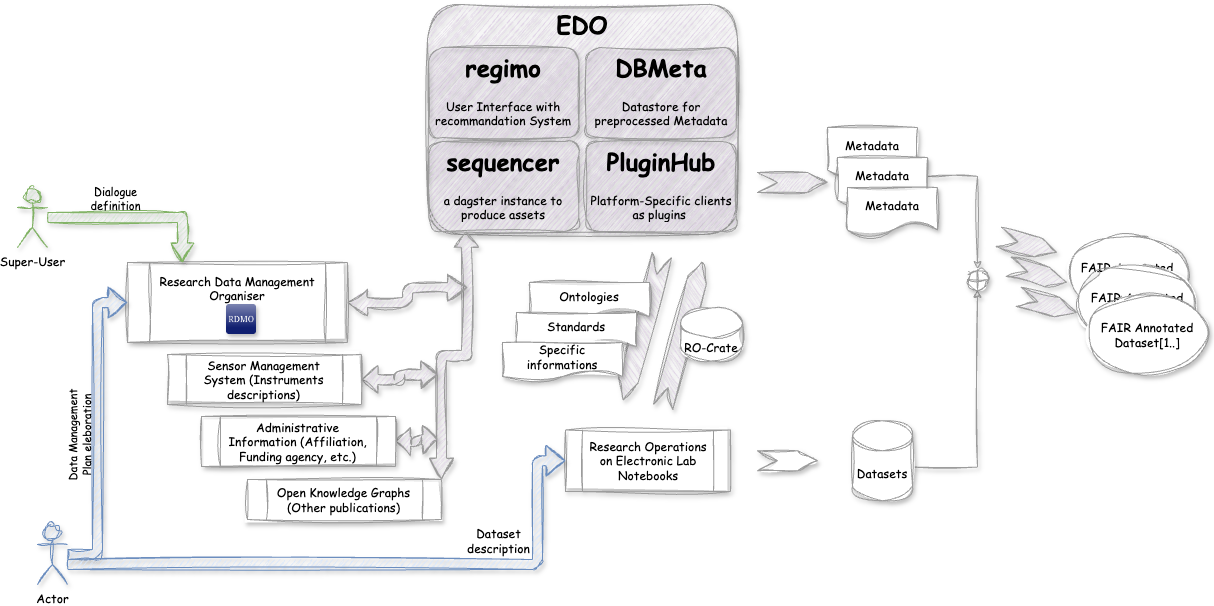
\includegraphics[width=.92\textwidth]{figs/fig_d1p3/edo_overview.png}
    \end{center}    
\end{frame}

\begin{frame}{The Research Data Lifecycle}
\begin{columns}[t]
    \begin{column}{0.5\textwidth}
            \begin{enumerate}
    \item \textbf{Plan \& Active Design:} Establishing actionable, machine-actionable Data Management Plans (maDMPs) at project onset to automate downstream metadata schema design and governance rules.
    \item \textbf{Capture \& Annotate:} Automating the collection, enrichment, and transformation of raw research data into structured datasets using FAIR-compliant, semantic metadata pipelines.

            \end{enumerate}
        \end{column}
        \begin{column}{0.5\textwidth}
    \begin{center}
    \vspace{-1.6cm} % Pulls the graph upwards 
    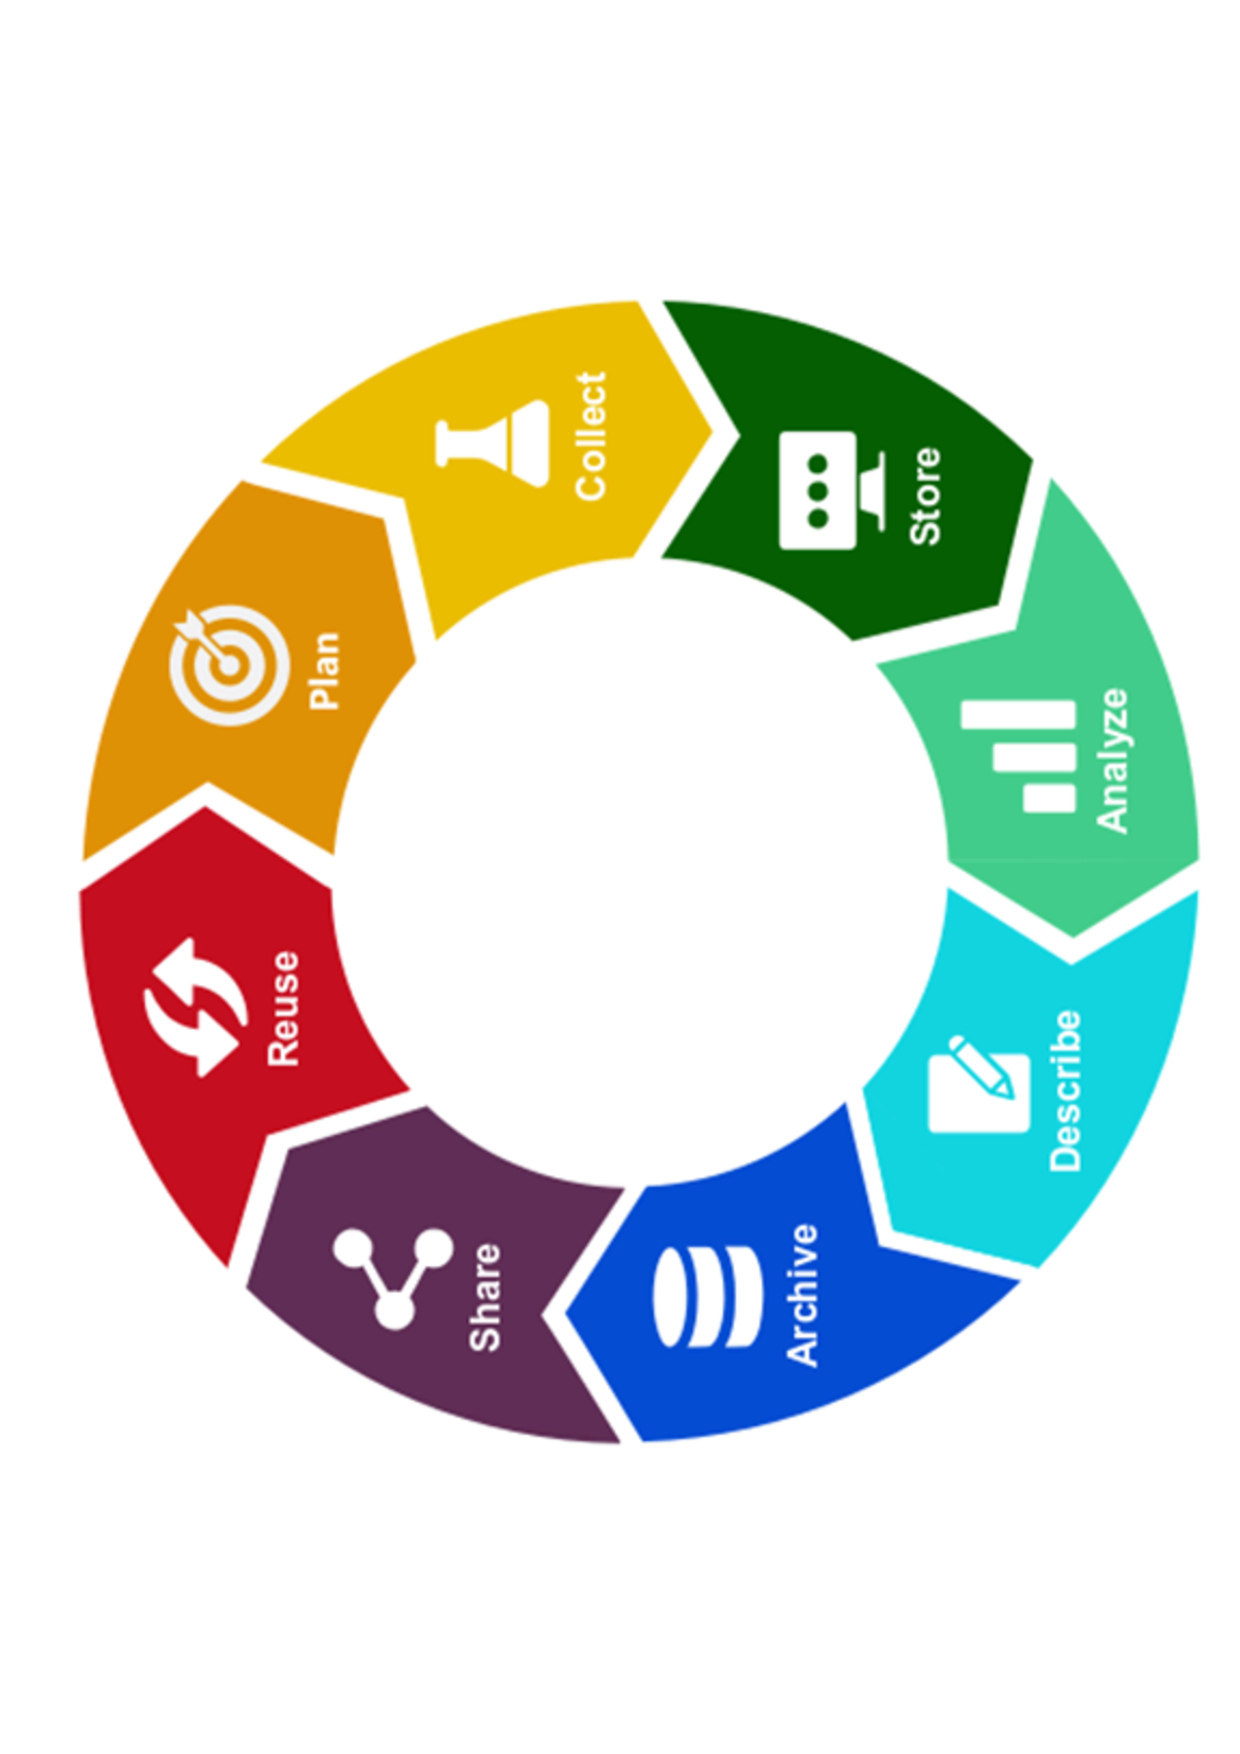
\includegraphics[width=.8\textwidth, angle=-90, ]{figs/retreat/Zyklus_en_2022_background_74a9925199.png.webp.pdf}
    \end{center}
\end{column}
\end{columns}
\end{frame}

\begin{frame}{The Research Data Lifecycle}
\begin{columns}[t]
    \begin{column}{0.5\textwidth}
            \begin{enumerate}
            \setcounter{enumi}{2}
    \item \textbf{Publish \& Disseminate:} Streamlining the deposit of annotated datasets into trusted repositories with persistent identifiers (PIDs) to ensure immediate discoverability.
    \item \textbf{Preserve \& Reuse:} Archiving well-described datasets for long-term preservation, allowing external researchers and automated systems to seamlessly find, access, and reuse the data.

            \end{enumerate}
        \end{column}
        \begin{column}{0.5\textwidth}
    \begin{center}
    \vspace{-1.6cm} % Pulls the graph upwards 
    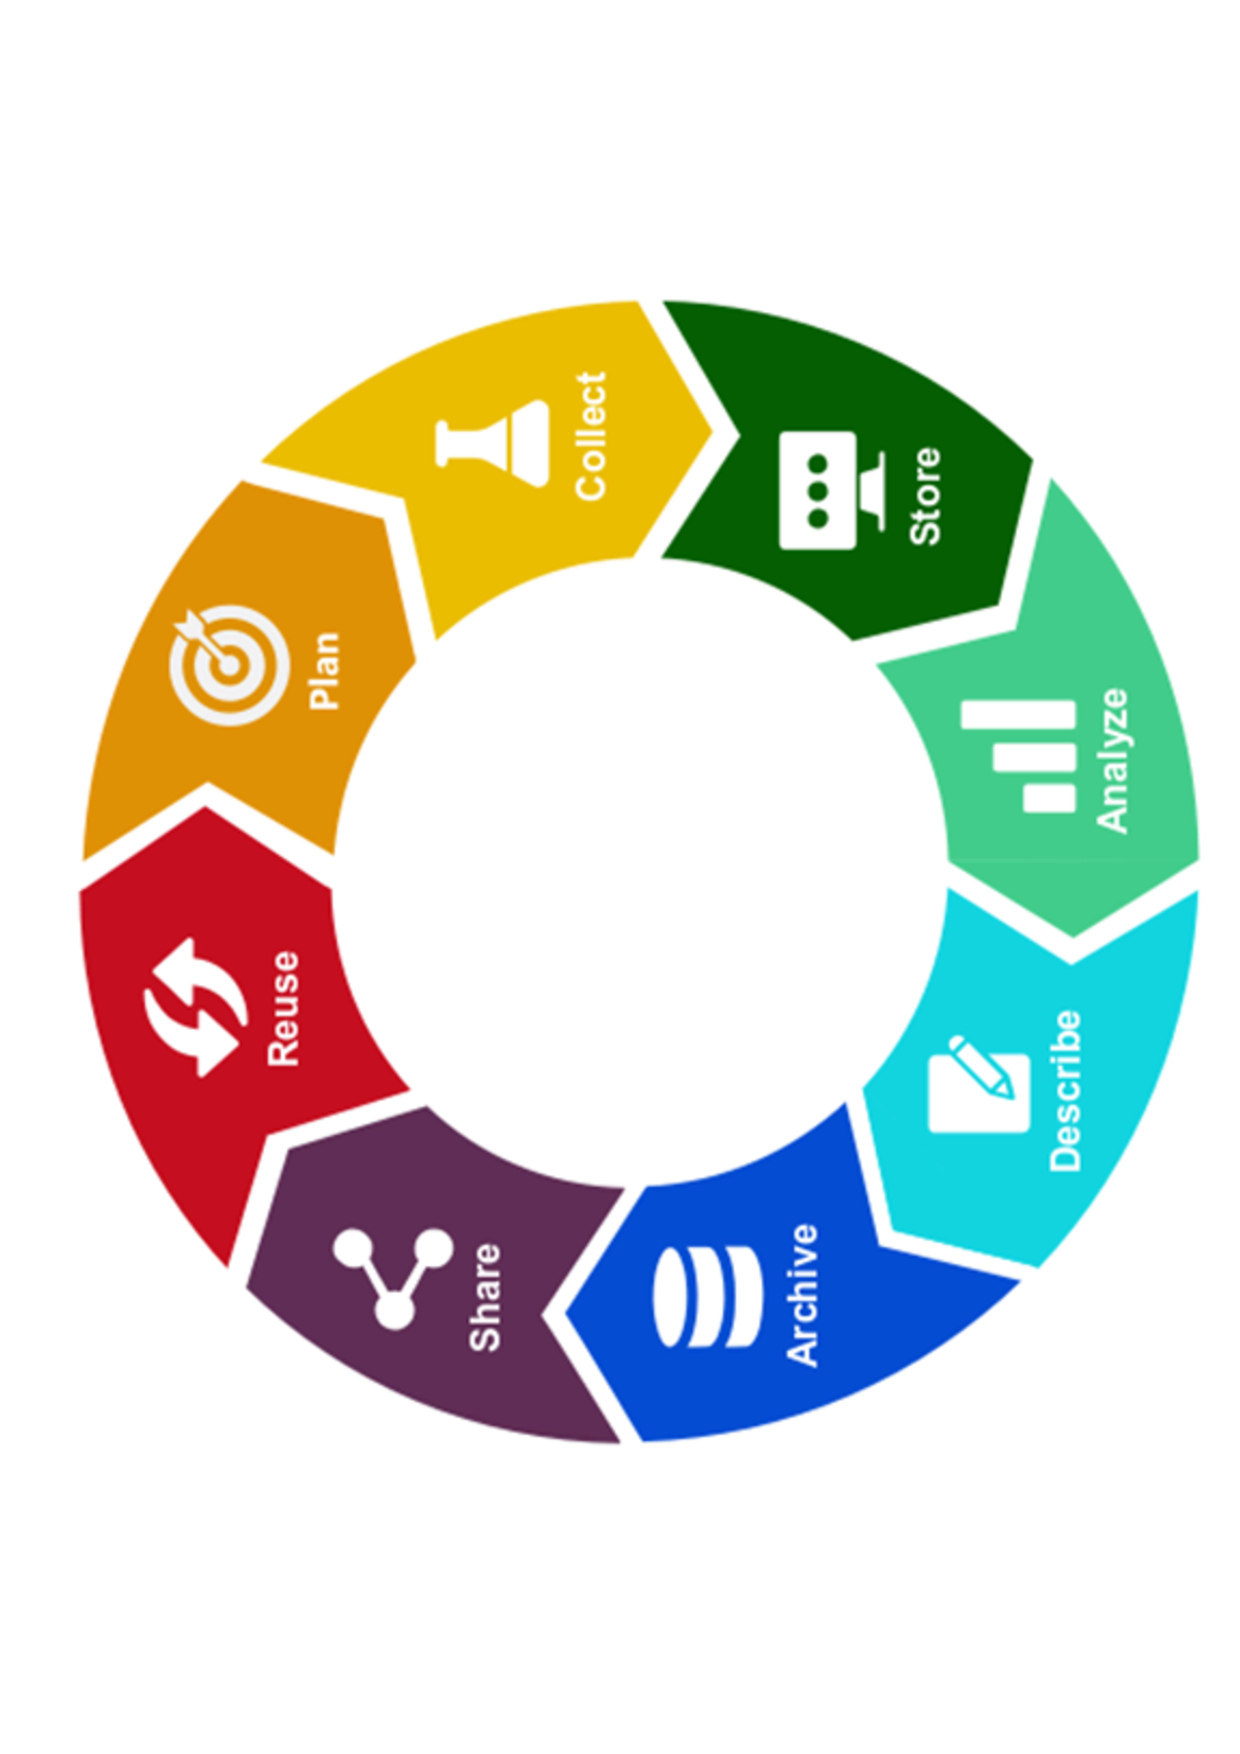
\includegraphics[width=.8\textwidth, angle=-90, ]{figs/retreat/Zyklus_en_2022_background_74a9925199.png.webp.pdf}
    \end{center}
\end{column}
\end{columns}
\end{frame}


\begin{frame}{Motivation}
\begin{columns}[t]
    \begin{column}{0.5\textwidth}
            \begin{enumerate}
    \item \textbf{Open License:} Make data available on the Web in whatever format (PDF, scanned image, TXT) under an open, reusable license.
    \item \textbf{Structured Data:} Provide the data in a machine-readable structured format (e.g., an Excel sheet instead of an image scan of a table).
            \end{enumerate}
        \end{column}
        \begin{column}{0.5\textwidth}
    \begin{center}
        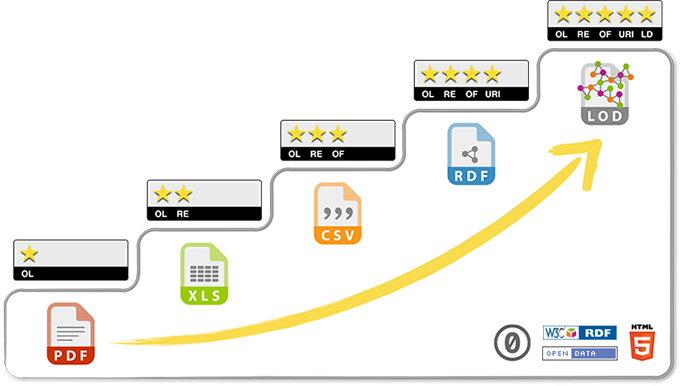
\includegraphics[width=.8\textwidth]{figs/fig_d1p1/5-star-steps.png}
    \end{center}    
 \end{column}
\end{columns}
\end{frame}
\begin{frame}{Motivation}
\begin{columns}[t]
    \begin{column}{0.5\textwidth}
            \begin{enumerate}
            \setcounter{enumi}{2}
    \item \textbf{Open Formats:} Publish in non-proprietary structured file formats (e.g., Comma-Separated CSV instead of locked proprietary XLS).
    \item \textbf{URIs for Things:} Use global HTTP Uniform Resource Identifiers (URIs) to name data points, allowing anyone to point directly to them.
            \end{enumerate}
        \end{column}
        \begin{column}{0.5\textwidth}
    \begin{center}
        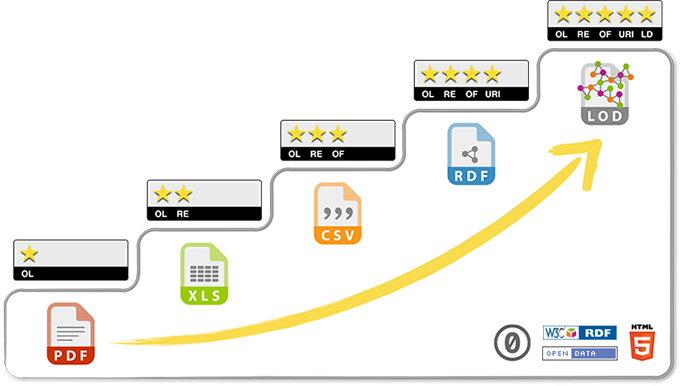
\includegraphics[width=.8\textwidth]{figs/fig_d1p1/5-star-steps.png}
    \end{center}    
 \end{column}
\end{columns}
\end{frame}
\begin{frame}{Motivation}
\begin{columns}[t]
    \begin{column}{0.5\textwidth}
            \begin{enumerate}
            \setcounter{enumi}{4}
    \item \textbf{Linked Context:} Link your own data items directly to other external datasets to provide global context, meaning, and discovery.
            \end{enumerate}
        \end{column}
        \begin{column}{0.5\textwidth}
    \begin{center}
        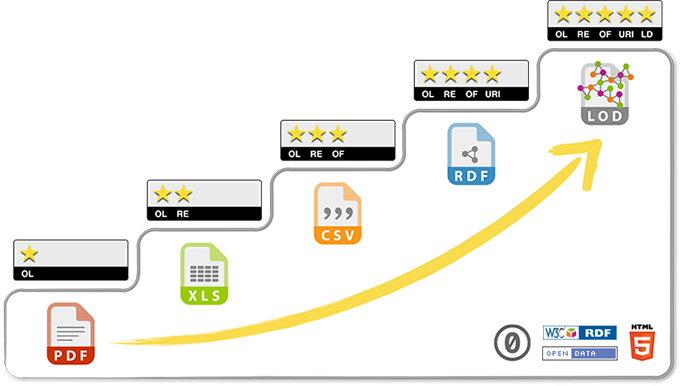
\includegraphics[width=.8\textwidth]{figs/fig_d1p1/5-star-steps.png}
    \end{center}    
 \end{column}
\end{columns}
\end{frame}

\begin{frame}{Why RO-Crate for Automated Enrichment?}
\begin{columns}[t]
    \begin{column}{0.64\textwidth}
    \begin{itemize}
        \item \textbf{JSON-LD Native:} Enables effortless machine parsing and automated metadata updates.
        \item \textbf{Standard Structure:} The predictable \texttt{ro-crate-metadata.json} provides a clear target for enrichment scripts.
        \item \textbf{Semantic Mapping:} Integrates \textit{Schema.org} to bind datasets to global ontologies automatically.
        \item \textbf{Context Packaging:} Bundles data and metadata together, ensuring context is never lost during pipeline hops.
    \end{itemize}
            \end{column}
        \begin{column}{0.36\textwidth}\begin{center}
        \vspace{0.64cm}
        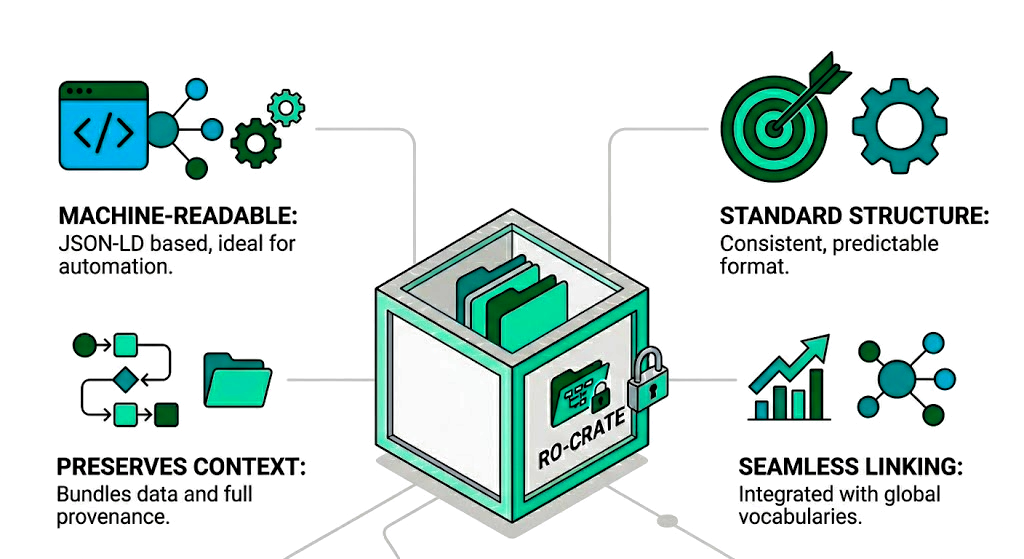
\includegraphics[width=\textwidth]{figs/retreat/ro-crate.png}
    \end{center}    
 \end{column}
\end{columns}
\end{frame}

% \begin{frame}{The Vision}
%     \begin{center}
%         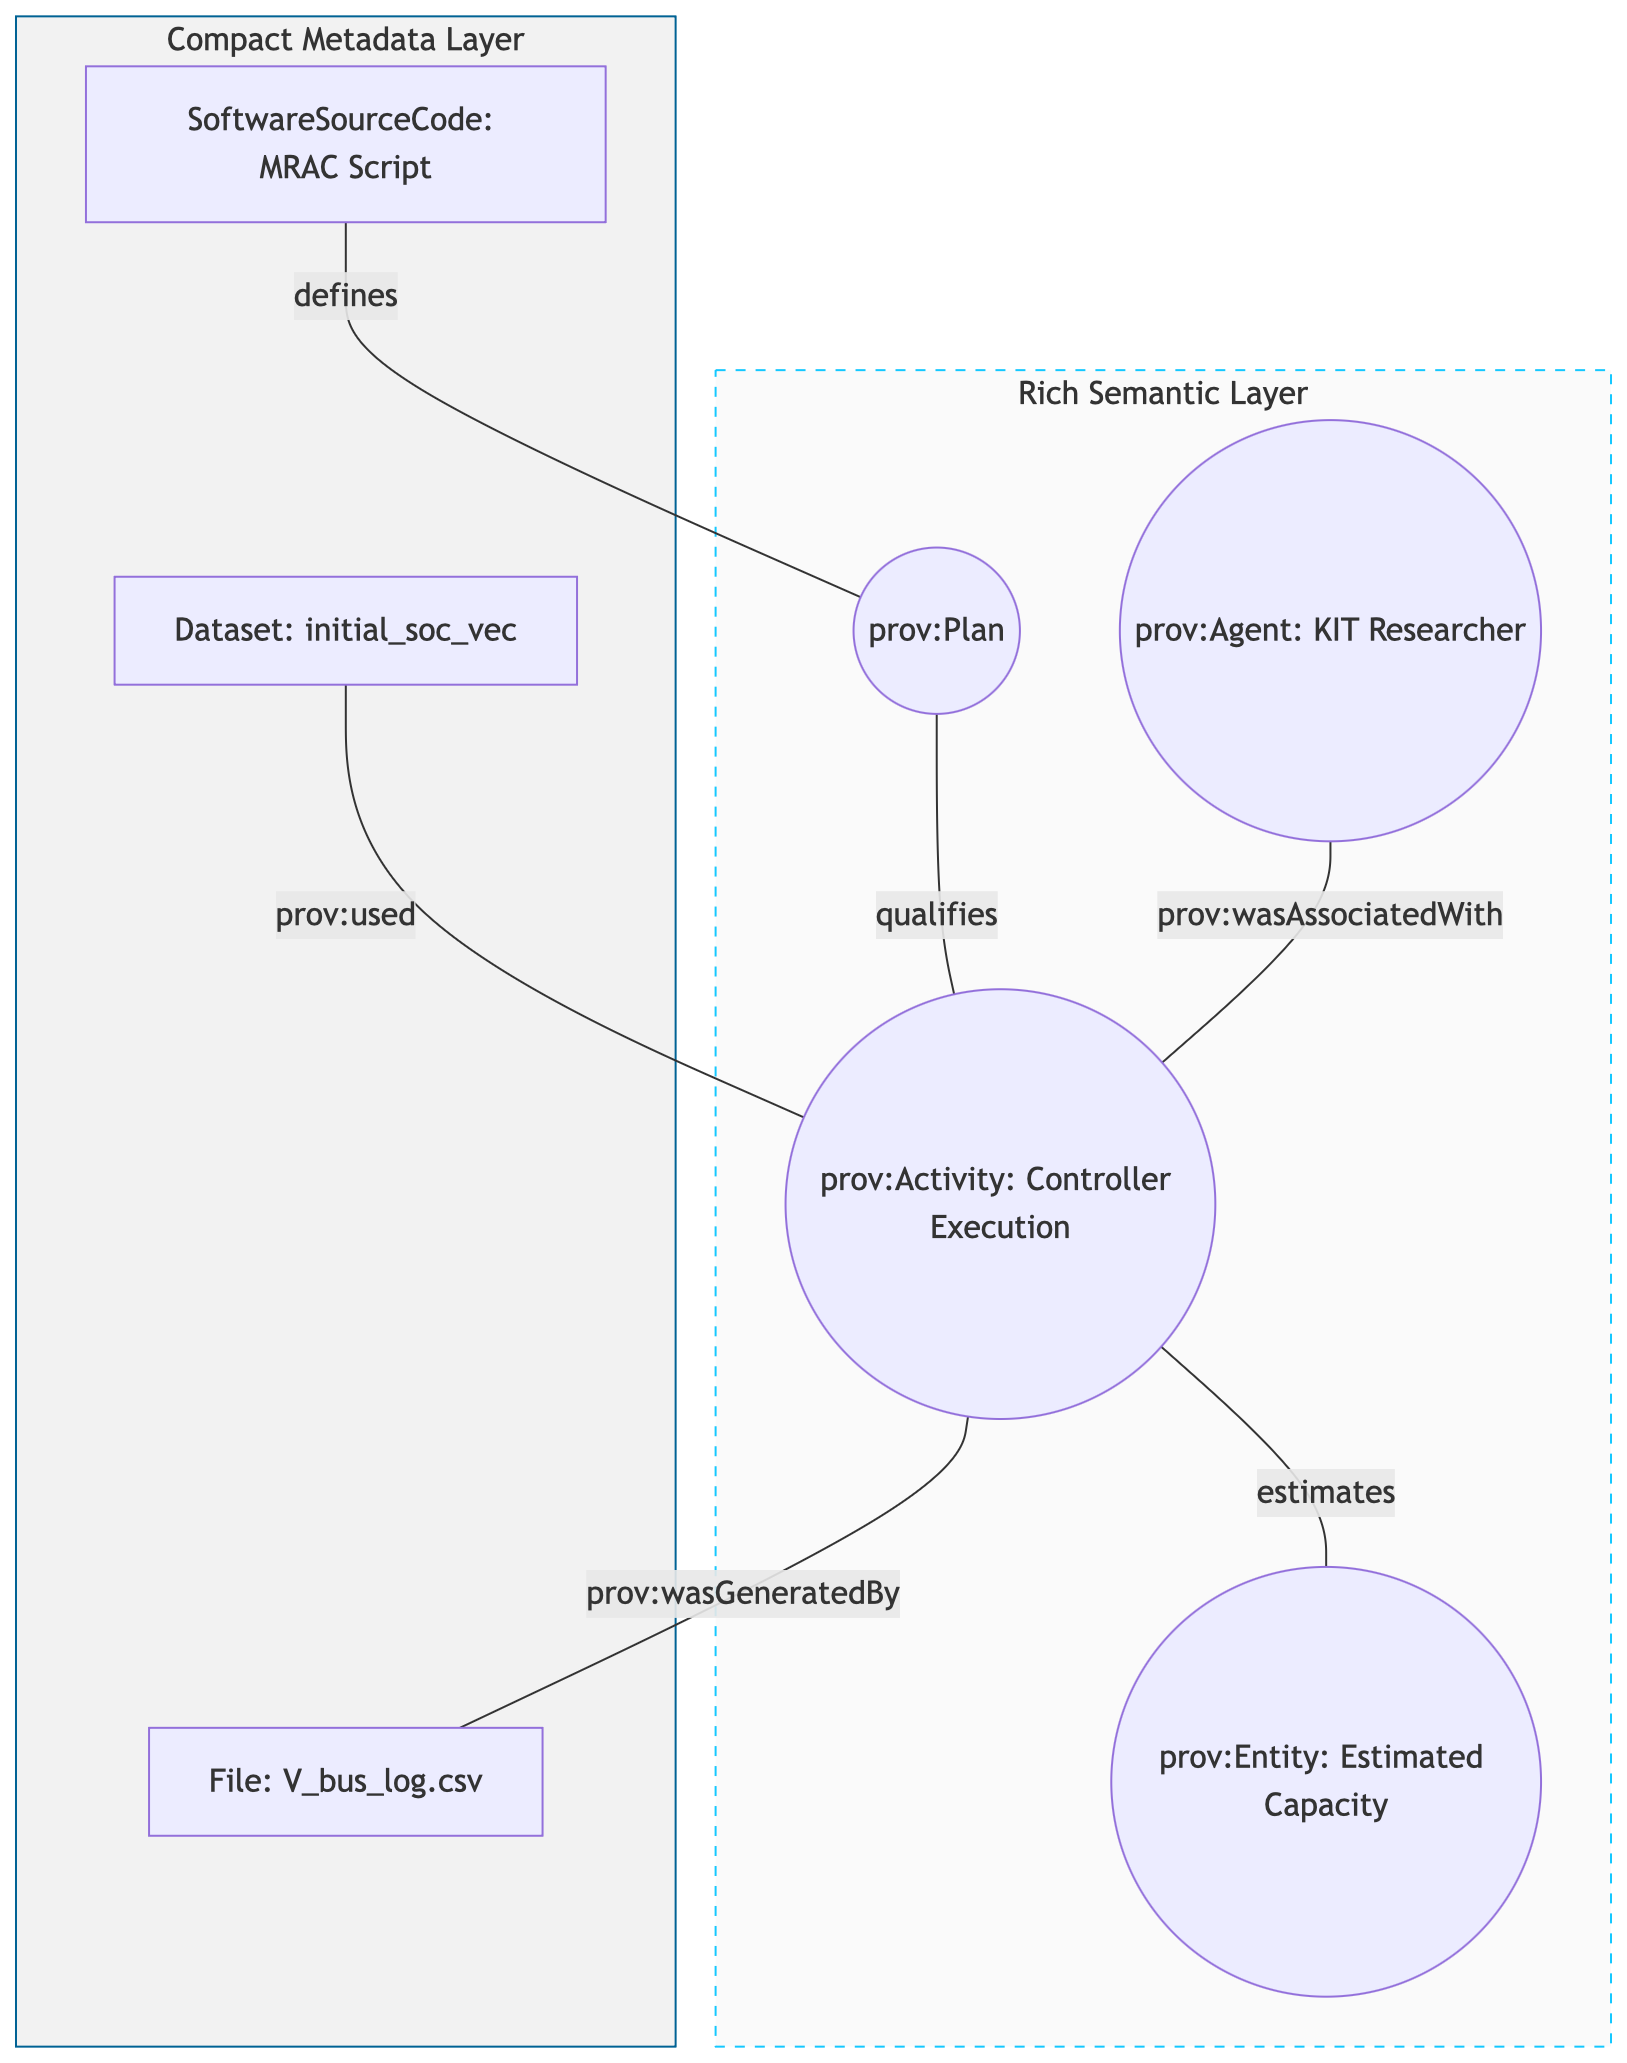
\includegraphics[width=.32\textwidth]{figs/colloquium/model_953.png}
%     \end{center}
% \end{frame}

\begin{frame}{RDA Machine-Actionable DMPs (maDMPs)}
    \begin{itemize}
        \item \textbf{Beyond Static Text:} Transforms traditional, narrative PDFs into structured, machine-interpretable JSON metadata models.
        \item \textbf{Common Standard:} Utilises the official RDA DMP Common Standard, establishing an open ecosystem for automated data exchanges.
        \item \textbf{Infrastructure Integration:} Enables automated systems (repositories, tools, and networks) to dynamically query and update project parameters.
        \item \textbf{Automated Workflows:} Triggers downstream orchestration—such as automatically configuring storage quotas or pre-populating dataset annotations.
    \end{itemize}
\end{frame}

\begin{frame}[plain]
  \vfill
  \centering
  \begin{beamercolorbox}[wd=\textwidth,center,sep=1em]{titlepage}
    \usebeamerfont{subtitle}\insertsubtitle\par
    \vspace{0.8em}
    \usebeamerfont{title}{\inserttitle}\par
    \vspace{1.5em}
    
    % Visual representation of the two spaces
    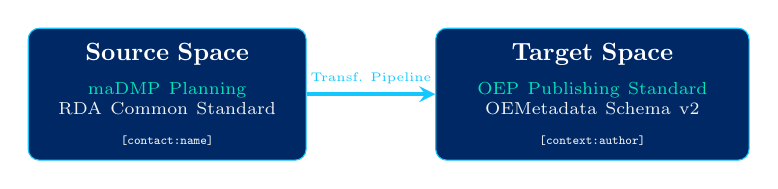
\begin{tikzpicture}[scale=0.9, every node/.style={transform shape}]
      \node[draw=HMCAccent, fill=HMCBlue, rounded corners, inner sep=6pt, text width=3.5cm, align=center] (source) at (0,0) {
        \textcolor{white}{\textbf{Source Space}}\\[2mm]
        \scriptsize\textcolor{HMCMint}{maDMP Planning}\\
        \textcolor{LightGray}{RDA Common Standard}\\
        \tiny\textcolor{LightGray}{\texttt{[contact:name]}}
      };
      
      \node[draw=HMCAccent, fill=HMCBlue, rounded corners, inner sep=6pt, text width=4cm, align=center] (target) at (6,0) {
        \textcolor{white}{\textbf{Target Space}}\\[2mm]
        \scriptsize\textcolor{HMCMint}{OEP Publishing Standard}\\
        \textcolor{LightGray}{OEMetadata Schema v2}\\
        \tiny\textcolor{LightGray}{\texttt{[context:author]}}
      };
      
      \draw[-stealth, line width=1.5pt, draw=HMCAccent] (source) -- node[above, text=HMCAccent, font=\tiny] {Transf. Pipeline} (target);
    \end{tikzpicture}
    
  \end{beamercolorbox}
  \vfill
\end{frame}

\begin{frame}{Schema-to-Schema vs. Canonical Data Model}
  \begin{columns}[t]
    \begin{column}{0.48\textwidth}
      \begin{block}{1. Schema-to-Schema Mapping}
        \scriptsize
        \textbf{Syntactic Translation} for static, well-defined spaces (e.g., relational, JSON/XML schemas).
        \vspace{0.5em}
        \begin{itemize}
          \item \textbf{How it works:} Define explicit translation mappings directly from source elements to target elements (e.g., ETL, XSLT, Liquid templates).
          \item \textbf{\textcolor{HMCMint}{Pros:}} High batch processing efficiency, low runtime overhead.
          \item \textbf{\textcolor{red!70}{Cons:}} Brittle design; breaks and requires manual maintenance whenever either schema changes.
        \end{itemize}
      \end{block}
    \end{column}
    
    \begin{column}{0.48\textwidth}
      \begin{block}{2. Mediated / Canonical Data Model}
        \scriptsize
        \textbf{CDM Strategy} decoupled from internal structures, ideal for scaling past two spaces.
        \vspace{0.5em}
        \begin{itemize}
          \item \textbf{How it works:} Source schemas are parsed into a universally understood neutral format (the canonical model) before translating to targets.
          \item \textbf{\textcolor{HMCMint}{Pros:}} Scale-friendly ($N$ data spaces without point-to-point explosion).
          \item \textbf{\textcolor{red!70}{Cons:}} High initial complexity in drafting a universally standard canonical model.
        \end{itemize}
      \end{block}
    \end{column}
  \end{columns}
\end{frame}

\begin{frame}{Semantic Brokerage vs. Metadata-Driven}
  \begin{columns}[t]
    \begin{column}{0.48\textwidth}
      \begin{block}{3. Semantic Brokerage}
        \scriptsize
        \textbf{Ontology Alignment} focusing on the preservation of meaning and FAIR data integrity.
        \vspace{0.5em}
        \begin{itemize}
          \item \textbf{How it works:} Local schemas are lifted into shared semantic spaces by mapping to structural/foundational ontologies (RDF, OWL, JSON-LD).
          \item \textbf{\textcolor{HMCMint}{Pros:}} Enables dynamic logic, reasoning; highly robust to schema modifications.
          \item \textbf{\textcolor{red!70}{Cons:}} Steeper initial overhead; requires domain expertise in Graph technologies.
        \end{itemize}
      \end{block}
    \end{column}
    
    \begin{column}{0.48\textwidth}
      \begin{block}{4. Metadata-Driven Orchestration}
        \scriptsize
        \textbf{Dynamic Execution} where the flow is validated and controlled by runtime parameters.
        \vspace{0.5em}
        \begin{itemize}
          \item \textbf{How it works:} Transfers carry machine-readable descriptors (LinkML, SHACL shapes). Ingestion pipelines automatically validate, shape, and route payloads.
          \item \textbf{\textcolor{HMCMint}{Pros:}} Minimal pipeline maintenance; natively supports validation \& quality audits.
          \item \textbf{\textcolor{red!70}{Cons:}} Demands a sophisticated, accessible registry configuration.
        \end{itemize}
      \end{block}
    \end{column}
  \end{columns}
\end{frame}

\begin{frame}{Application: From Planning (maDMP) to Publication (OEP)}
  \begin{itemize}
    \item \textbf{The Core Pipeline Challenge:}\\[1mm]
    Translating intent-driven data definitions (maDMP) into standard tabular schemas on publishing portals like the \textbf{Open Energy Platform (OEP)} using the \textbf{OEMetadata Standard}.
  \end{itemize}
  \vspace{0.5em}
  \centering
  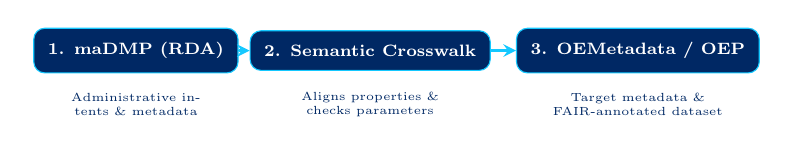
\begin{tikzpicture}[scale=0.85, every node/.style={transform shape}]
    \draw[dashed, draw=HMCMint] (0, 1.2) -- (10, 1.2);
    
    \node[fill=HMCBlue, text=white, rounded corners, draw=HMCAccent, inner sep=6pt] (p1) at (1, 1.2) {\scriptsize \textbf{1. maDMP (RDA)}};
    \node[fill=HMCBlue, text=white, rounded corners, draw=HMCAccent, inner sep=6pt] (p2) at (4.5, 1.2) {\scriptsize \textbf{2. Semantic Crosswalk}};
    \node[fill=HMCBlue, text=white, rounded corners, draw=HMCAccent, inner sep=6pt] (p3) at (8.5, 1.2) {\scriptsize \textbf{3. OEMetadata / OEP}};
    
    \draw[-stealth, draw=HMCAccent, line width=1pt] (p1) -- (p2);
    \draw[-stealth, draw=HMCAccent, line width=1pt] (p2) -- (p3);
    
    \node[text=HMCBlue, font=\tiny, text width=3cm, align=center] at (1, 0.4) {Administrative intents \& metadata};
    \node[text=HMCBlue, font=\tiny, text width=3.2cm, align=center] at (4.5, 0.4) {Aligns properties \& checks parameters};
    \node[text=HMCBlue, font=\tiny, text width=3cm, align=center] at (8.5, 0.4) {Target metadata \& FAIR-annotated dataset};
  \end{tikzpicture}
\end{frame}

\begin{frame}{Strategy Selection Matrix}
  \centering
  \scriptsize
  \renewcommand{\arraystretch}{1.2}
  \begin{tabular}{l p{2.2cm} p{2.2cm} p{2.2cm} p{2.2cm}}
    \toprule
    \textbf{Criterion} & \textbf{Schema-to-Schema} & \textbf{Canonical Model} & \textbf{Semantic Brokerage} & \textbf{Metadata-Driven} \\
    \midrule
    \textbf{Complexity} & Low & Medium & High & Medium-High \\
    \arrayrulecolor{HMCBlue}\hline
    \textbf{Flexibility}  & Low & Medium & Very High & High \\
    \arrayrulecolor{HMCBlue}\hline
    \textbf{Best Used For} & One-off or static point-to-point transfers & Enterprise system integrations ($N$ data spaces) & Interdisciplinary or evolving domains (FAIR) & Dynamic, automated data pipelines \\
    \bottomrule
  \end{tabular}
\end{frame}

\begin{frame}{Conclusion: Choosing the Optimal Strategy}
  \centering
  \begin{minipage}{0.85\textwidth}
    \begin{block}{Evaluating The Architecture}
      The final decision on selecting a strategic mechanism boils down to defining the scope and agility of the collaborative network:
    \end{block}
    \vspace{0.8em}
    \begin{itemize}
      \item \textbf{Is the environment a static, closed ecosystem?} \\
      If yes, simple \textcolor{HMCAccent}{\textbf{Schema-to-Schema mappings}} or standard \textcolor{HMCAccent}{\textbf{Canonical models}} are highly effective and keep overhead minimum.
      \vspace{0.8em}
      \item \textbf{Is a flexible, FAIR-compliant, automated pipeline required?} \\
      If schemas, variables, and licensing criteria alter frequently per dataset, opt for \textcolor{HMCAccent}{\textbf{Semantic Brokerage}} or \textcolor{HMCAccent}{\textbf{Metadata-Driven Orchestration}} to resolve integration conflicts automatically.
    \end{itemize}
  \end{minipage}
\end{frame}

\begin{frame}{Semantic Brokerage: Mediating Meaning via Ontologies}
    
    \begin{columns}[c]
        \begin{column}{0.56\textwidth}
            \begin{block}{Why Use a Broker?}
                \scriptsize
                \begin{itemize}
                    \item \textbf{Meaning $>$ Syntax:} Focuses on \textit{what} the data is (concept), not \textit{how} it is stored (format).
                    \item \textbf{Decoupled Systems:} Source and Target never need to know each other's schema.
                    \item \textbf{Resilient to Change:} If OEP updates its schema, only the Broker's mapping is updated—not the sources.
                    \item \textbf{Dynamic Reasoning:} Automatically resolves synonyms (e.g., \texttt{is\_author} $\equiv$ \texttt{creator}).
                \end{itemize}
            \end{block}
            
            \vspace{0.3cm}
            \centering
            \tikz \draw[fill=HMCAccent!20, draw=HMCAccent] (0,0) rectangle (0.2,0.2); 
            \tiny \textcolor{HMCAccent}{\textbf{FAIR COMPLIANT (I \& R)}}
        \end{column}
        \begin{column}{0.44\textwidth}
            \centering
            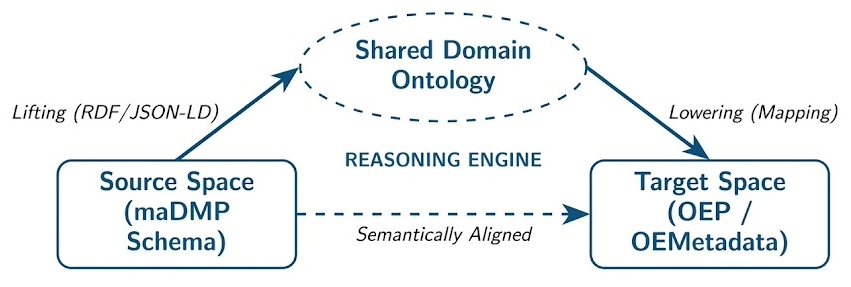
\includegraphics[width=\textwidth]{figs/retreat/Brokerage.png}
            
            \vspace{0.4cm}
            \scriptsize{Pattern: Local schemas are lifted into a neutral graph based on global URIs, ensuring meaning is preserved over structure.}
        \end{column}
    \end{columns}
\end{frame}

% ============

\begin{frame}{The Provenance Audit Framework}
    \framesubtitle{Structural Verification of Executable Research Objects}
    
    \begin{block}{Discovery \& Integrity Layers}
        \begin{itemize}
            \item Resolves \texttt{prov:Activity} from RO-Crate metadata to establish context.
            \item Executes physical checksum verification (e.g., \texttt{V\_bus\_log.csv}) against metadata hashes to ensure data immutability.
        \end{itemize}
    \end{block}

    \begin{block}{Logical \& Temporal Layers}
        \begin{itemize}
            \item Validates \texttt{prov:hadPlan} to verify the \texttt{Est} function’s adaptive control logic.
            \item Uses \texttt{prov:startedAtTime} and \texttt{prov:endedAtTime} to confirm the $T_{sim} = 2400$s window.
        \end{itemize}
    \end{block}

    \vfill
    \centering
    \textit{Goal: Certify execution as a deterministic result of logic applied to data.}
\end{frame}

\begin{frame}{The Isolated Execution Layer}
    \framesubtitle{Guaranteeing Redoability through Architectural Parity}
    
    \begin{exampleblock}{Trusted Execution Environment (TEE)}
        Instantiates a containerised sandbox.
    \end{exampleblock}

    \begin{columns}[t]
        \begin{column}{0.5\textwidth}
            \textbf{Reproduction Workflow}
            \begin{enumerate}
                \item \textbf{Injection:} Permits only \texttt{prov:used} entities to eliminate bias.
                \item \textbf{Reproduction:} Triggers \texttt{prov:Plan} for MRAC adaptation.
                \item \textbf{Validation:} Cross-references outputs using tolerance $\epsilon$.
            \end{enumerate}
        \end{column}
        \begin{column}{0.5\textwidth}
            \textbf{Scientific Impact}
            \begin{itemize}
                \item Ensures estimated plant parameters converge consistently.
                \item Validates total storage capacity estimation across environments.
            \end{itemize}
        \end{column}
    \end{columns}
\end{frame}

\begin{frame}{Integrating RO-Crate and PROV-O}
    \begin{itemize}
        \item \textbf{RO-Crate:} A community-driven method for packaging research data with structured metadata (JSON-LD).
        \item \textbf{PROV-O:} The W3C Provenance Ontology providing a model to map the origins of data.
        \item \textbf{The Goal:} Use RO-Crate to store the "What" (data/tools) and PROV-O to describe the "How" (process/execution).
    \end{itemize}
    \vspace{0.3cm}
    \begin{block}{Core PROV-O Relationships}
        \begin{itemize}
            \item \texttt{prov:Entity}: Data objects or software within the crate.
            \item \texttt{prov:Activity}: The computation or manual step performed.
            \item \texttt{prov:Agent}: The researcher or system responsible.
        \end{itemize}
    \end{block}
\end{frame}

\begin{frame}{Linking Entities for Traceability}
    To make operations verifiable, the RO-Crate \texttt{ro-crate-metadata.json} must link files to their execution context:
    \vfill
    \begin{enumerate}
        \item \textbf{wasGeneratedBy}: Links a result file (\textit{Entity}) to a specific script run (\textit{Activity}).
        \item \textbf{used}: Links the activity to its input datasets and parameter files.
        \item \textbf{wasAssociatedWith}: Connects the activity to the \textit{Agent} (e.g., a KIT research fellow) or a software environment.
    \end{enumerate}
    \vfill
    \textit{Benefit:} This graph allows a machine to traverse from a plot back to the exact version of the raw data and code used.
\end{frame}

\begin{frame}{Enabling Re-runnability and Parameterisation}
    \begin{itemize}
        \item \textbf{Verifiability:} Independent auditors can check if the \texttt{prov:Activity} outputs match the provided \texttt{prov:Entity}.
        \item \textbf{Redoability:} By describing the \texttt{SoftwareApplication} as a \texttt{prov:Plan}, others can swap input entities.
        \item \textbf{Parameter Tracking:} Store configuration files as \texttt{prov:Entity} linked via the \texttt{used} property.
    \end{itemize}
    \begin{exampleblock}{Workflow Logic}
        If a researcher wants to test a new parameterisation, they identify the \texttt{Activity} in the RO-Crate, substitute the input \texttt{Entity}, and re-execute the linked \texttt{SoftwareSourceCode}.
    \end{exampleblock}
\end{frame}

\begin{frame}{PIDINST: Persistent Identification of Instruments}
    \framesubtitle{Anchoring Hardware Metadata in PROV-O}
    
    \begin{block}{The Role of PIDINST}
        \begin{itemize}
            \item Assigns a \textbf{Persistent Identifier (DOI/Handle)} to physical instruments (e.g., Battery Cyclers, Sensors).
            \item Provides machine-readable metadata: Manufacturer, Model, Serial Number, and Calibration History.
        \end{itemize}
    \end{block}

    \begin{block}{PROV-O Integration}
        \begin{itemize}
            \item \textbf{prov:Agent:} The instrument acts as an automated agent performing an activity.
            \item \textbf{prov:Entity:} Represents the instrument state at the time of simulation.
            \item Enables the Auditor to verify if the hardware used (e.g., in Karlsruhe) matches the specifications required by the \texttt{prov:Plan}.
        \end{itemize}
    \end{block}
\end{frame}

\begin{frame}{The Persistent Identifier (PID) Ecosystem}
    \framesubtitle{Interconnected Metadata for Verifiable Research}
    
    \begin{center}
        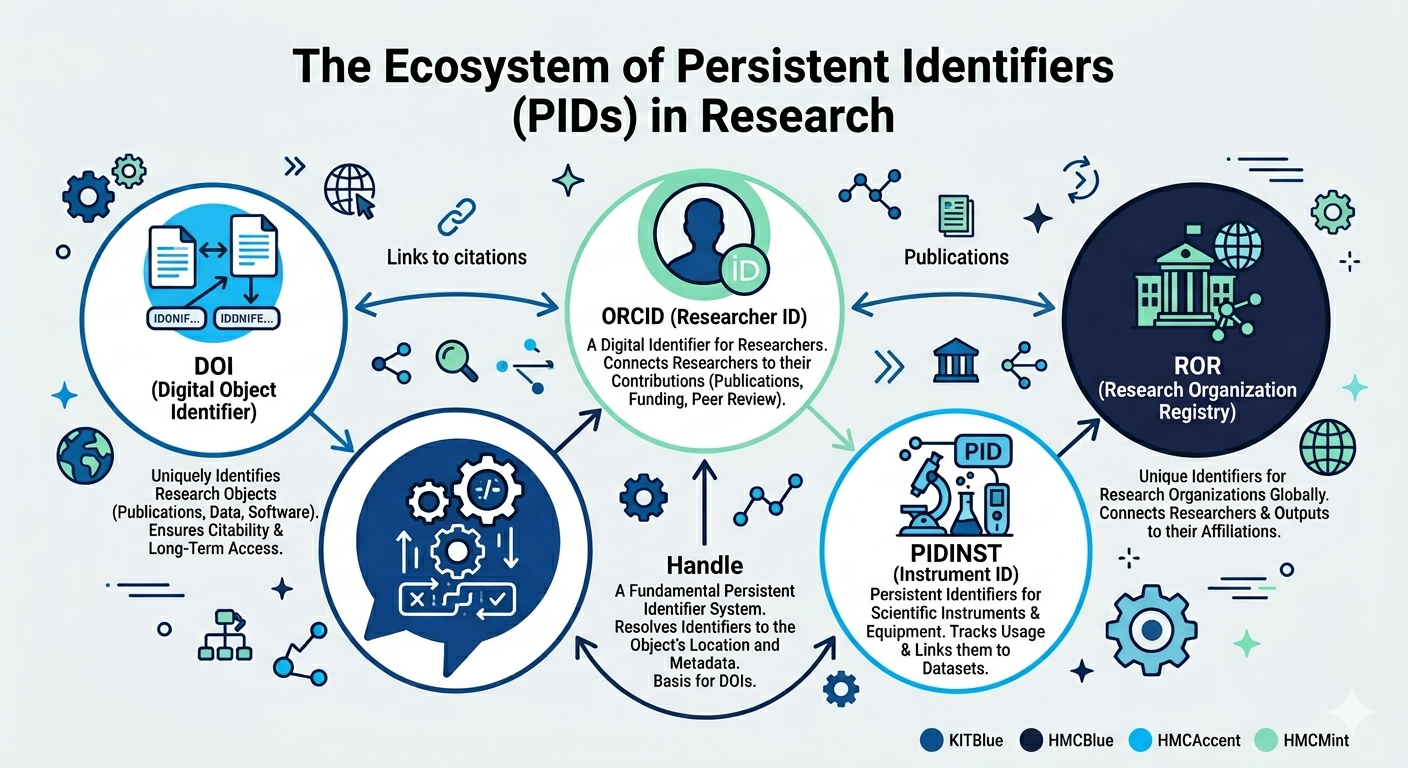
\includegraphics[width=0.32\textwidth]{figs/colloquium/pids.png}
    \end{center}

    \begin{columns}[t]
        \begin{column}{0.48\textwidth}
            \small
            \textbf{Core Infrastructure:}
            \begin{itemize}
                \item \textbf{ORCID/ROR:} Link researchers and their affiliations.
                \item \textbf{DOI/Handle:} Ensure long-term citability of datasets and software.
            \end{itemize}
        \end{column}
        \begin{column}{0.48\textwidth}
            \small
            \textbf{Experimental Context:}
            \begin{itemize}
                \item \textbf{PIDINST:} Connects physical instruments to the \texttt{prov:Activity}.
                \item \textbf{Graph Utility:} Enables a reachness of information across the audit chain.
            \end{itemize}
        \end{column}
    \end{columns}
\end{frame}

\begin{frame}{PIDINST}
\begin{columns}
        \column{.36\textwidth}
        \begin{center}
            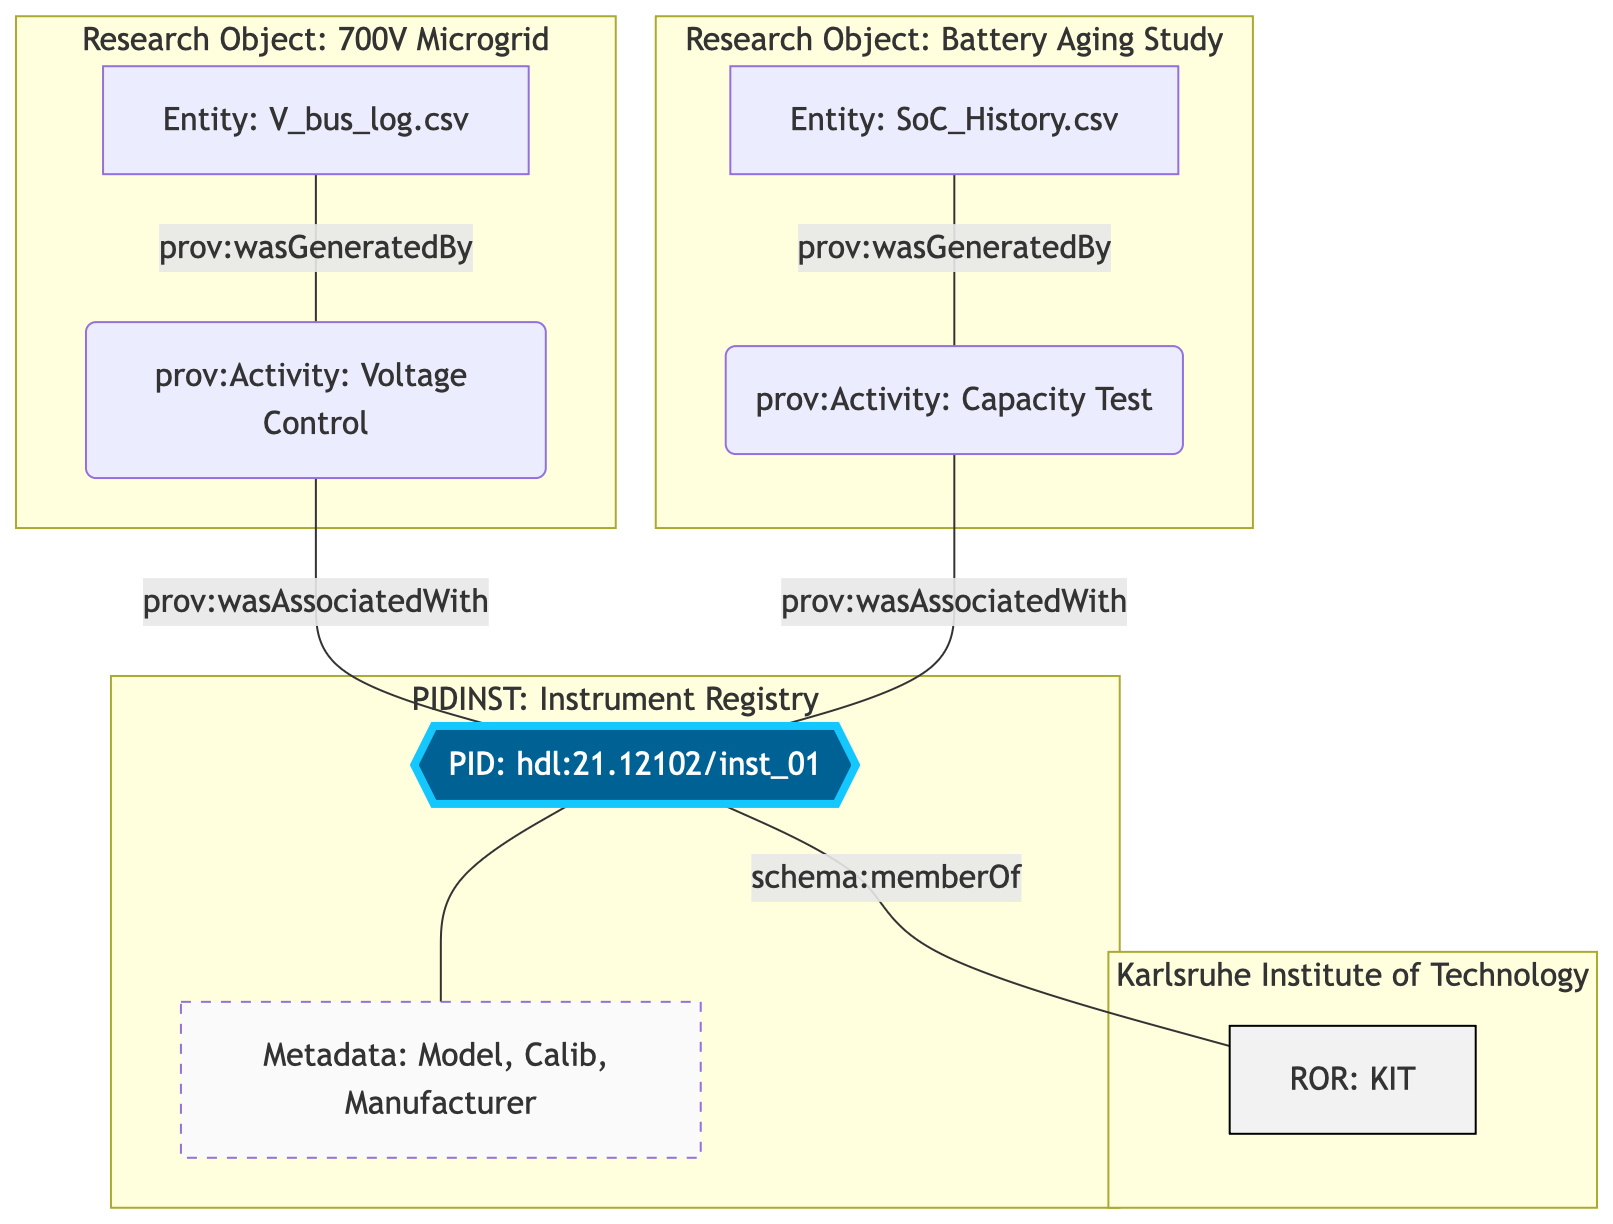
\includegraphics[width=.8\textwidth]{figs/colloquium/example_pid_807.png}
        \end{center}
        \column{.64\textwidth}
        \begin{center}
            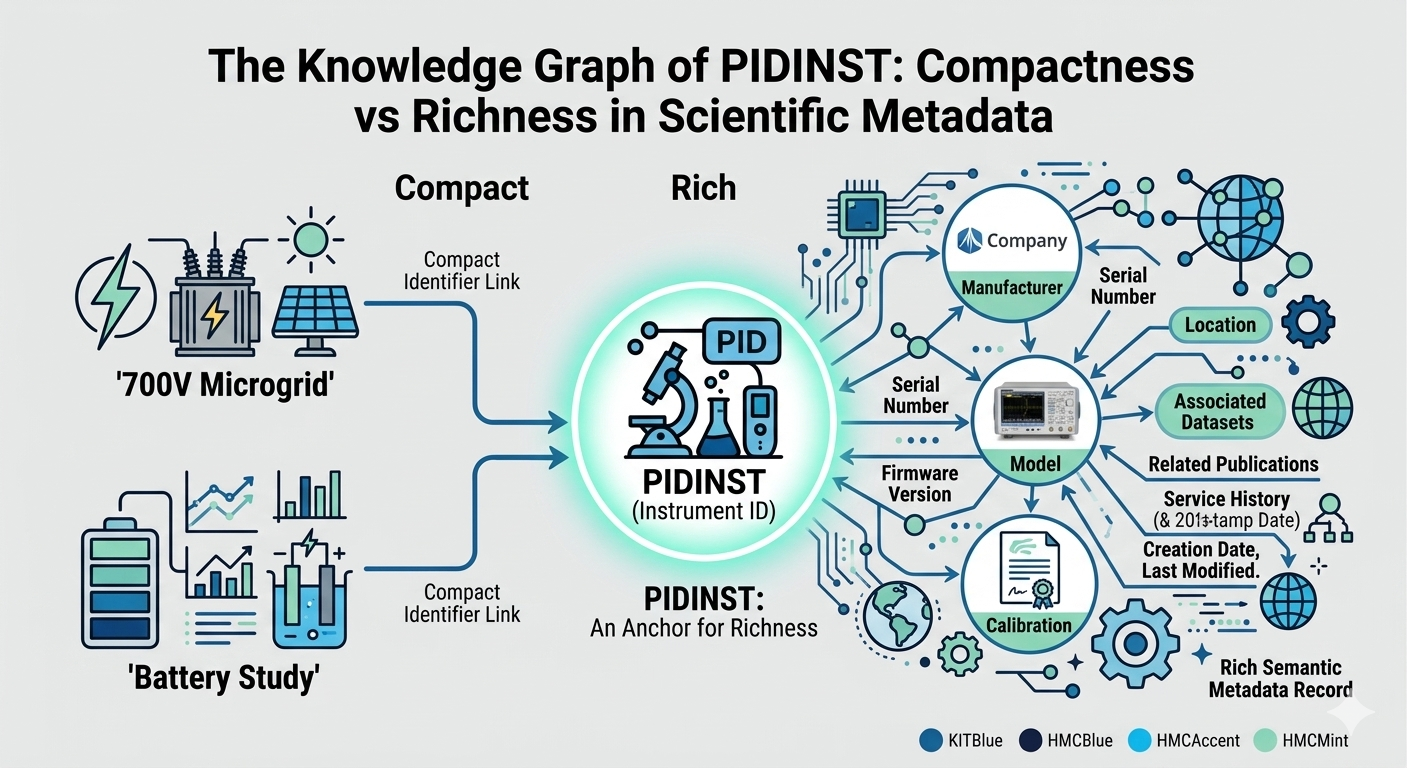
\includegraphics[width=.8\textwidth]{figs/colloquium/compactness.png}
        \end{center}
\end{columns}
    
\end{frame}

% Defining Graph Density and Structural Compactness
\begin{frame}{1. Structural Compactness vs. Density}
    % \framesubtitle{Mathematical Foundation of Metadata Efficiency}
    \begin{block}{Graph Density ($D$)}
        For a graph with $V$ vertices and $E$ edges, density represents the ratio of actual connections to potential ones:
        \[ D = \frac{|E|}{|V|(|V|-1)} \]
    \end{block}
    \begin{itemize}
        \item \textbf{The PIDINST Effect:} By substituting internal metadata clusters (redundant nodes for serial numbers, models, and calibration) with a single URI, we reduce $|E|$ and $|V|$ locally.
        \item \textbf{Theorem:} A more compact graph minimizes $D$ while maintaining the \textit{Reachability} of information.
    \end{itemize}
    \vfill
    \centering
    \textit{Question: At what point does a graph become too sparse to be self-describing?}
\end{frame}

% Slide 2: Semantic Entropy and Information Content
\begin{frame}{2. Semantic Entropy and Richness}
    % \framesubtitle{Quantifying the "Diversity" of Provenance}
    \begin{block}{Graph Entropy ($H$)}
        Based on Shannon's theory, we measure the complexity of the semantic distribution:
        \[ H(G) = -\sum_{i=1}^{n} P(\text{rel}_i) \log_b P(\text{rel}_i) \]
    \end{block}
    \begin{itemize}
        \item \textbf{Richness Factor:} High richness is defined by a diverse set of PROV-O relations (\texttt{used}, \texttt{wasInformedBy}, \texttt{hadPlan}).
        \item \textbf{Optimization:} Using PIDs increases $H(G)$ per node, as each node carries higher "Significance" within the network topology.
    \end{itemize}
    \vfill
    \centering
    \textit{Discussion: Does increasing entropy always improve reproducibility?}
\end{frame}

% Slide 3: Betweenness Centrality and Bridge Nodes
\begin{frame}{3. Centrality and The "Bridge" Effect}
    % \framesubtitle{PIDs as High-Utility Hubs}
    \begin{block}{Betweenness Centrality ($C_B$)}
        Measures the extent to which a node lies on paths between others:
        \[ C_B(v) = \sum_{s \neq v \neq t} \frac{\sigma_{st}(v)}{\sigma_{st}} \]
    \end{block}
    \begin{itemize}
        \item \textbf{PIDINST as a Hub:} In an institutional graph at KIT, PIDINST identifiers exhibit the highest $C_B$, acting as the "glue" between disparate Research Objects.
        \item \textbf{Verification Efficiency:} The Auditor/Orchestrator can reach the context or the \textit{MRAC} logic faster by traversing these high-centrality nodes.
    \end{itemize}
    \vfill
    \centering
    \textit{Question: Does reliance on central hubs create a single point of failure for EDO?}
\end{frame}

% Slide 4: The Convergence of Logic and Data
\begin{frame}{4. Discussion: The Efficiency of Truth}
    \framesubtitle{Towards a Unified Metric for Executable Research Objects}
    \begin{itemize}
        \item \textbf{The Compactness-Richness Paradox:} We seek to minimize the "Data Footprint" of the RO-Crate while maximizing its "Logical Depth."
        \item \textbf{Proposed Discussion Points:}
        \begin{enumerate}
            \item Can we define a \textbf{Reproducibility Index} based on the average path length between a result and its PIDINST/Plan?
            \item How does architectural parity shift the graph from a \textit{Descriptive} state to an \textit{Executable} state?
            \item Should "FAIRness" be measured by the mathematical modularity of the institutional Knowledge Graph?
        \end{enumerate}
    \end{itemize}
    \vfill
    \centering
    \textbf{Opening for Group Discussion}
\end{frame}

% Slide 1: The Mathematical Metric
\begin{frame}{Mathematical Modularity ($Q$) in the KG}
    \framesubtitle{Quantifying the Strength of Semantic Clusters}
    
    \begin{block}{The Modularity Formula}
        Modularity ($Q$) measures how much more "clustered" a graph is compared to a random distribution of edges:
        \[ Q = \frac{1}{2m} \sum_{ij} \left[ A_{ij} - \frac{k_i k_j}{2m} \right] \delta(c_i, c_j) \]
    \end{block}

    \begin{itemize}
        \item \textbf{$A_{ij}$}: Relationship between nodes $i$ and $j$.
        \item \textbf{$k$}: Degree of nodes (number of connections).
        \item \textbf{$\delta(c_i, c_j)$}: Limits the sum to nodes within the same community (e.g., your specific 700V microgrid simulation).
    \end{itemize}
    \vfill
    \centering
    \textit{High $Q$ indicates a "healthy" graph where data is logically compartmentalised.}
\end{frame}

% Slide 2: PIDINST as the Structural Driver
\begin{frame}{Structural Impact: PIDs vs. Redundancy}
    \framesubtitle{How PIDINST Protects Graph Modularity}
    
    \begin{columns}[t]
        \begin{column}{0.5\textwidth}
            \textbf{Without PIDINST}
            \begin{itemize}
                \item Metadata is duplicated across every experiment.
                \item \textbf{Result:} "Fuzzy" communities and lower $Q$.
                \item The graph becomes a "Big Ball of Mud."
            \end{itemize}
        \end{column}
        \begin{column}{0.5\textwidth}
            \textbf{With PIDINST}
            \begin{itemize}
                \item The instrument is a central hub \textit{between} clusters.
                \item \textbf{Result:} High internal density with strategic external links.
                \item Maximises $Q$ for the institutional graph.
            \end{itemize}
        \end{column}
    \end{columns}

    \begin{exampleblock}{The Reachness Paradox}
        We achieve higher \textbf{Reachness} (access to rich sensor data) while maintaining lower \textbf{Graph Density} within the Research Object.
    \end{exampleblock}
\end{frame}

% Slide 3: The Auditor's Perspective
\begin{frame}{Modularity in the Redoability Audit}
    \framesubtitle{Ensuring Scalability for the KIT Infrastructure}
    
    High modularity is essential for the \textbf{Orchestrator} when verifying an Executable Research Object (ERO):

    \begin{description}
        \item[Isolation:] The Auditor can extract the 700V microgrid provenance chain without "leakage" from unrelated battery ageing studies.
        \item[Search Efficiency:] Computational cost of pathfinding (from result to \texttt{prov:Plan}) remains low even as the Knowledge Graph grows.
        \item[Validation:] High $Q$ allows for automated consistency checks of the \textbf{MRAC} logic against the \textbf{Darwin ARM64} environment variables.
    \end{description}

    \vfill
    \centering
    \textbf{Discussion:} Should Modularity be an automated KPI for "FAIR" institutional data management?
\end{frame}

\end{document}

\begin{frame}{Closing: Task-Based Semantic Framework}
    \begin{itemize}
        \item \textbf{Conceptual Mapping:} Research processes are broken down into logical \enquote{Tasks} that map to \texttt{prov:Activity}.
        \item \textbf{Abstraction Levels:} Differentiates between a high-level scientific goal and the technical execution (scripts/tools).
        \item \textbf{The Semantic Gap:} Bridging the gap between raw data files and the scientific intent behind their manipulation.
    \end{itemize}
    \vspace{0.2cm}
    \begin{block}{Implementation Strategy}
        Use the RO-Crate to define a \texttt{SoftwareSourceCode} as a \texttt{prov:Plan}. An \texttt{Activity} is then \textit{qualified} by this plan, ensuring that the operation is not just recorded, but described by its intended logic.
    \end{block}
\end{frame}

% --- SLIDE 5: Automated vs. Manual Provenance ---
\begin{frame}{Automated vs. Manual Provenance Implementation}
    The framework addresses both \enquote{ideal} (automated) and \enquote{pragmatic} (manual) scenarios:
    \vfill
    \begin{columns}[T]
        \begin{column}{0.48\textwidth}
            \textbf{Automated (Ideal)}
            \begin{itemize}
                \item Tool-generated logs mapped to PROV-O.
                \item Precise timestamps and PID-linked entities.
                \item High granularity of parameters.
            \end{itemize}
        \end{column}
        \begin{column}{0.48\textwidth}
            \textbf{Manual (Pragmatic)}
            \begin{itemize}
                \item Human-recorded task descriptions.
                \item Linking \texttt{prov:Agent} (Researcher) to activities.
                \item Capturing environment state via \enquote{Shadow Metadata}.
            \end{itemize}
        \end{column}
    \end{columns}
    \vfill
    \begin{center}
        \textit{Crucial for Reproducibility: Even a manual \enquote{Data Cleaning} task must be an entity-linked Activity.}
    \end{center}
\end{frame}

% --- SLIDE 6: Verification & Executable Research Objects ---
\begin{frame}{Verification \& Executable Research Objects}
    By combining RO-Crate and PROV-O, the crate becomes a \textit{Self-Describing Research Object}:
    \begin{itemize}
        \item \textbf{Traceability:} One can traverse from a \texttt{prov:Entity} (Result) $\rightarrow$ \texttt{prov:Activity} (Operation) $\rightarrow$ \texttt{prov:Entity} (Input).
        \item \textbf{Integrity:} Checksums in the RO-Crate ensure the entities used in the provenance graph haven't been tampered with.
        \item \textbf{Verifiability:} Allows a KIT research fellow or external auditor to evaluate if the results are mathematically or logically consistent with the inputs.
    \end{itemize}
    \begin{exampleblock}{Conclusion}
        Linking entities via PROV-O within an RO-Crate shifts research from \textit{archiving} to \textit{active documentation}, making complex operations redoable and verifiable.
    \end{exampleblock}
\end{frame}

\end{document}
